\section{I/O}
The majority of the I/O infrastructure delivering diagnostic output in the form of UGRID-NetCDF via XIOS is on the LFRic trunk
and will be used as part of the Aquaplanet runs in 2019. Therefore it is now necessary to begin regular monitoring of the impact
of I/O on compute performance. In 2017, following the preliminary integration of XIOS into the LFRic infrastructure, performance
tests were done, focussing mainly on strong scaling of LFRic-XIOS for diagnostic output. The conclusion was that XIOS scaled well
out to 384 nodes (approx. 14K cores). A description of the work plus full results can be found in \cite{Adams2018}. 

For the 2019 report, the focus is on two main areas: strong scaling when outputting regular
diagnostics and also tests of in-situ post-processing. In particular tests have been done of time-meaning and also regridding 
from the LFRic native cubed-sphere mesh to a regular lat-lon mesh. Both of these are use cases from the upcoming Aquaplanet
runs and also evaluation of XIOS regridding is of interest to the wider Next Generation Modelling Systems programme as it
could inform how downstream processing will be handled. For instance whether LFRic can deliver Level 1 data directly to StaGE.
It could also make verification of LFRic easier if the data can be directly produced on a lat-lon mesh. The aim of the post-processing
experiments described here is primarily to get an idea of computational overhead in terms of runtime and memory, 
so there is no in depth analysis of scientific accuracy apart from verifying that the jobs have produced the right kind of output. 

\subsection{Job Setup}
All tests were performed on XCS. The executables were built using the LFRic Intel Fortran environment (17.0.0.098) 
including the latest PSyclone 1.7.0 and XIOS at r1537 of the XIOS trunk. Build flags were the default fast-debug.

The science configuration was the standard baroclinic wave test with timestep length dependent on mesh resolution. 
For the purposes of the tests here: 900s for a C96 mesh and 180s for a C576 mesh.
10 fields are currently output as diagnostics in this configuration which results in approximately 5 Gb data per
output

To keep within queue time limit the basic run is for 120 timesteps, with diagnostic frequency set to 20 timesteps.
This makes for 6 writes over the course of the run.

\subsection{Glossary of terms}

 
\begin{itemize}
  \item Client Ratio (CR).The percentage of time a client (model) task waits for the server. Ideally it should be as close to zero as possible.
  \item Client I/O time. The actual time (seconds) that the client task spends in I/O related activity
\end{itemize} 



\subsection{Set 1: Strong scaling}

This set of tests used a C576 mesh (approx 17Km horizontal resolution). Pure MPI only (\$OMP\_NUM\_THREADS=1). 
I/O setup used 12 XIOS servers with lustre stripe set count to be the same. This was the best performing setup from
the last set of I/O performance tests, so the assumption is that it is a good starting point.
The basic run is for 120 timesteps, with diagnostic\_frequency set to 20 timesteps. This makes for 6 writes over the course of the run.

\begin{table}[ht!]
\scriptsize
  \begin{center}
    \caption{Strong Scaling: Runtime}
    \label{tab:table1}
     \begin{tabular}{|c|c|c|c|c|c|}
      \textbf{Nodes} & \textbf{Max CR~(\%)} & \textbf{Max Client IO~(s)} & \textbf{Runtime~(s)} & \textbf{Runtime no IO~(s)} & \textbf{\% incr IO}\\
      \hline
      24 & 0.002 & 12.76 & 10115 & & \\
      54 & 0.002 & 13.30 & 4950 & & \\
      96 & 0.006 & 13.36 & 2795 & & \\
      216 & & & & & \\
      384 & & & & & \\
    \end{tabular}
  \end{center}
\end{table}

\begin{table}[ht!]
\scriptsize
  \begin{center}
    \caption{Strong Scaling: Memory Usage *}
    \label{tab:table2}
     \begin{tabular}{|c|c|c|}
      \textbf{Nodes} & \textbf{Memory Usage Gb} & \textbf{Memory Usage Gb (No IO)} \\
      \hline
      24 & 841.3 &  \\
      54 & 1020.2  &  \\
      96 & ? &  \\
      216 & & \\
      384 & & \\
    \end{tabular}
  \end{center}
\end{table}

\scriptsize \textbf{* Note some job output does not include the PBS epilogue and so memory usage is not available (indicated by ?)}
\newline

\normalsize
The results are very similar to those done in the 2016/2017 tests (which were done with a C288 mesh). For the 24, 54 and 96 node jobs we see
evidence that scaling is preserved from the decreasing run times. The Client Ratio (CR) is very close to zero in all cases, 
showing that model client tasks are hardly waiting at all for I/O requests to be processed and that I/O is asynchronous.

\textbf{Comment on \% increase of runtime and memory usage over non I/O jobs when results are available.}

216 and 384 node jobs crashed out within the first few timesteps with XIOS-related errors even though no I/O was
actually happening at those timesteps. I am assuming that further tuning is needed for these higher node-count jobs.
See the Conclusions section for suggested avenues to explore.

\subsection{Set 2: In-situ Post-processing}

In this set the focus is on regridding and simple time-meaning, with usage examples taken from latest Aquaplanet branch.
The aim here is to get an idea of computational overhead in terms of runtime and memory, and general correctness rather than scaling.
Therefore, these tests were done with a lower-resolution C96 mesh and only out to 96 nodes.
Runs have also been done to compare run time and memory usage to the same job configuration with only regular diagnostic output and also 
no I/O to get an idea of the additional penalty for using XIOS post-processing. 

\subsubsection{Averaging}

As Set 1, with the following changes: C96 mesh, 900s timestep.
In addition to regular diagnostics, averages are output over 20 timesteps, giving 6 writes to an additional file. 

\normalsize
\begin{figure}[ht!]
  \begin{center}
   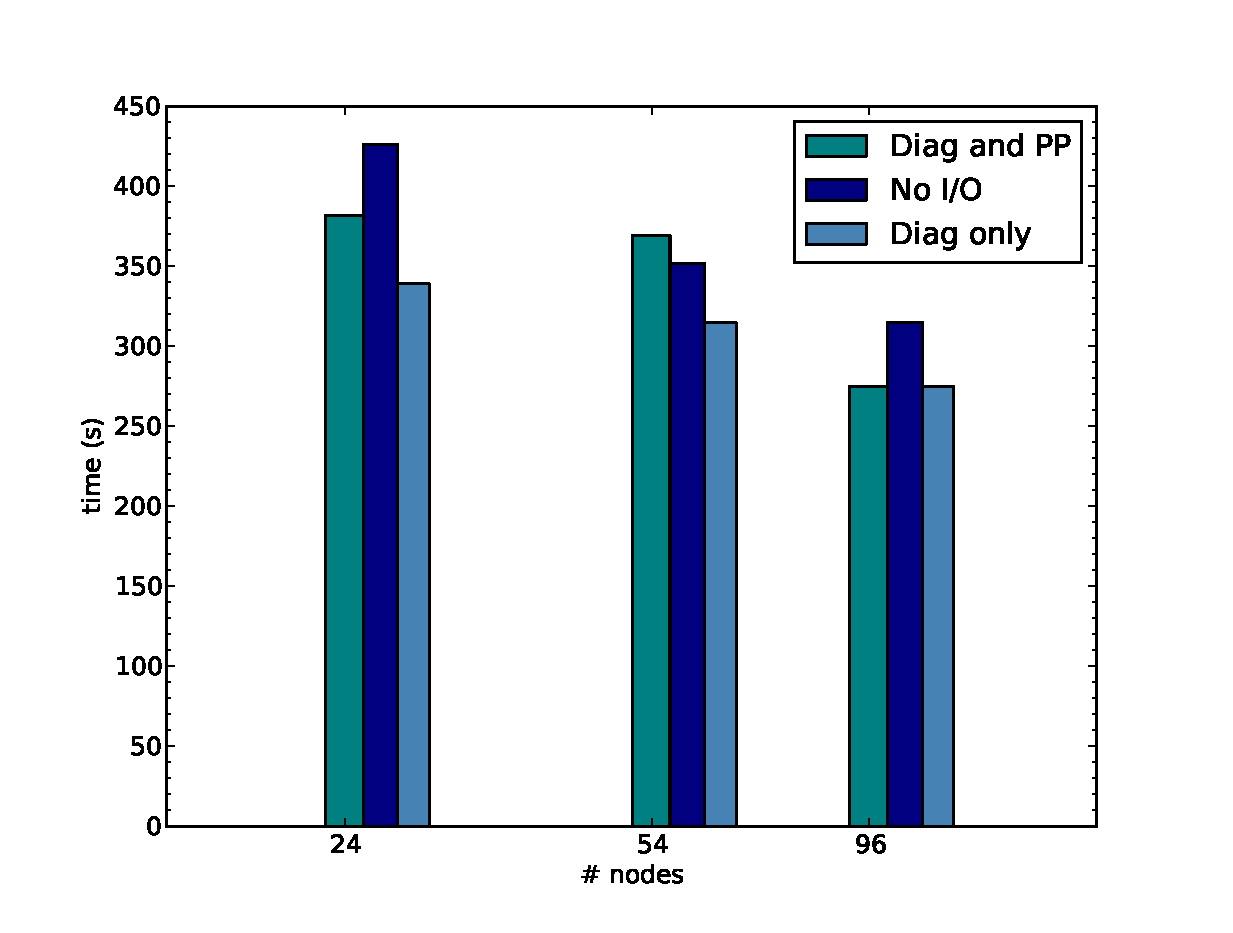
\includegraphics[scale=0.4]{figs/ave.eps}
   \caption{Averaging}
   \label{fig:fig1}
  \end{center}
\end{figure}

\begin{table}[ht!]
\scriptsize
  \begin{center}
    \caption{Averaging: Runtime}
    \label{tab:table3}
     \begin{tabular}{|c|c|c|c|c|c|}
      \textbf{Nodes} & \textbf{Max CR~(\%)} & \textbf{Max Client IO~(s)} & \textbf{Runtime~(s)} & \textbf{\% incr diag IO} & \textbf{\% incr no IO}\\
      \hline
      24 & 0.02 & 1.63 & 382 & -11 & +11 \\ 
      54 & 0.03 & 0.90 & 369 & +5 & +19 \\ 
      96 & 0.04 & 2.90 & 275 & -14 & 0 \\ 
    \end{tabular}
  \end{center}
\end{table}

\begin{table}[ht!]
\scriptsize
  \begin{center}
    \caption{Averaging: Memory Usage}
    \label{tab:table4}
     \begin{tabular}{|c|c|c|c|}
      \textbf{Nodes} & \textbf{Memory Usage Gb (pp) } & \textbf{Memory Usage Gb (diag only)} & \textbf{Memory Usage Gb (no IO)} \\
      \hline
      24 & 82.9 & 81.8 & 77.4 \\
      54 & 150.9 & 149.2 & 138.8 \\
      96 & 234.1 & ? & ? \\
    \end{tabular}
  \end{center}
\end{table}


Figure \ref{fig:fig1} gives a quick overview of scaling comparing run times for jobs without I/O, with regular diagnostic output and with
regular diagnostic output plus averaging. Scaling is still evident as run times generally decrease with the number of nodes. From
Table \ref{tab:table3}, the \% increases over just diagnostic output and no I/O are inconclusive - sometimes positive and sometimes negative. 
The range seems to be greater than for Set 1 so maybe a 5-10\% runtime penalty can be inferred, but it is difficult to say 
without doing runs to assess run time variability. Table \ref{tab:table4} shows a clear memory usage increase when adding different types of I/O. 
About +6-7\% for diagnostic I/O over runs with no I/O and a further +1\% for adding averaging post-processing. 


\subsubsection{Regridding}

As Set 1, with the following changes: C96 mesh, 900s timestep.
In addition to regular diagnostics, the rho, exner and divergence fields are regridded (to N96 equivalent) and output every 20ts, giving 6 writes to an additional file. Two sets of runs were done: computing weights on-the-fly each time and also using precomputed weights.

\normalsize
\begin{figure}[ht!]
  \begin{center}
   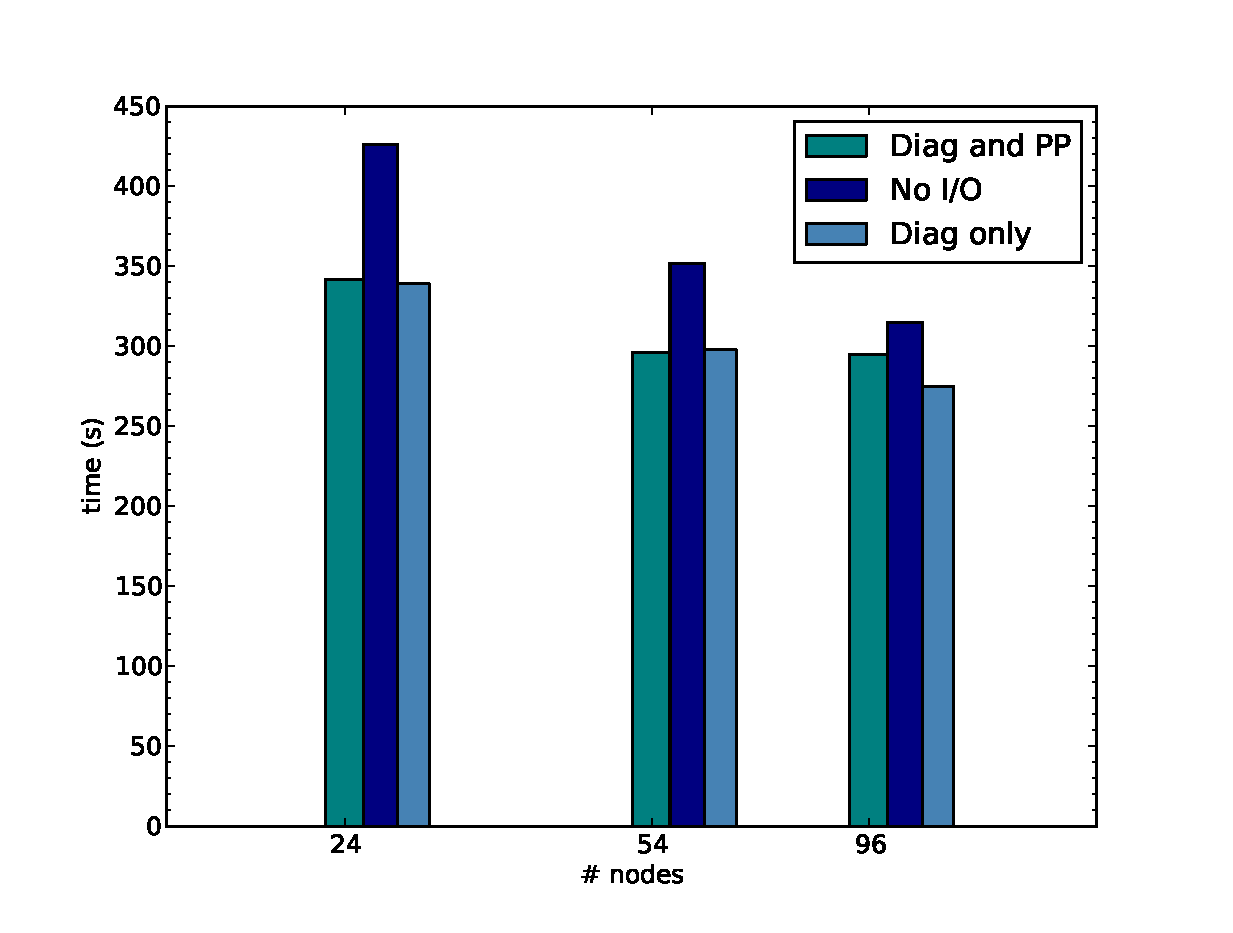
\includegraphics[scale=0.4]{figs/regrid.eps}
   \caption{Regridding (computing weights)}
   \label{fig:fig2}
  \end{center}
\end{figure}

\begin{figure}[ht!]
  \begin{center}
   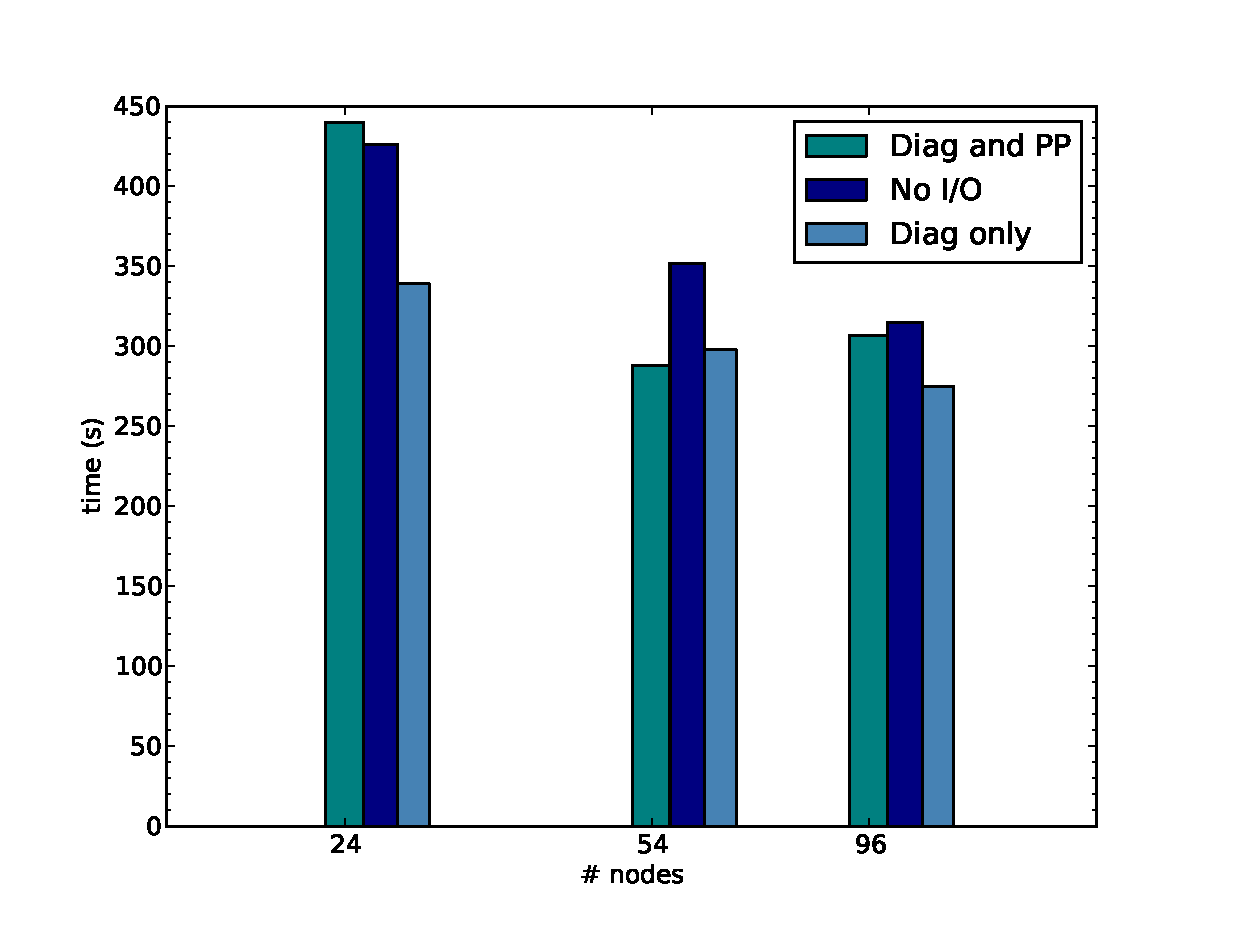
\includegraphics[scale=0.4]{figs/regrid_pcw.eps}
   \caption{Regridding (precomputed weights)}
   \label{fig:fig3}
  \end{center}
\end{figure}

\begin{table}[ht!]
\scriptsize
  \begin{center}
    \caption{Regrid, computing weights: Runtime}
    \label{tab:table5}
     \begin{tabular}{|c|c|c|c|c|c|}
      \textbf{Nodes} & \textbf{Max CR~(\%)} & \textbf{Max Client IO~(s)} & \textbf{Runtime~(s)} & \textbf{\% incr diag IO} & \textbf{\% incr no IO}\\
      \hline
      24 & 0.03 & 9.10 & 342 & -24 & +0.9 \\ 
      54 & 0.04 & 9.89 & 296 & -19 & -0.6 \\
      96 & 0.05 & 17.01 & 295 & -7 & +7 \\
    \end{tabular}
  \end{center}
\end{table}

\begin{table}[ht!]
\scriptsize
  \begin{center}
    \caption{Regrid, computing weights: Memory Usage}
    \label{tab:table6}
     \begin{tabular}{|c|c|c|c|}
      \textbf{Nodes} & \textbf{Memory Usage Gb (pp) } & \textbf{Memory Usage Gb (diag only)} & \textbf{Memory Usage Gb (no IO)} \\
      \hline
      24 & 83.0 & 81.8 & 77.4 \\
      54 & 150.6 & 149.2 & 138.8 \\
      96 & ? & ? & ? \\
    \end{tabular}
  \end{center}
\end{table}

\begin{table}[ht!]
\scriptsize
  \begin{center}
    \caption{Regrid, precomputed weights: Runtime}
    \label{tab:table7}
     \begin{tabular}{|c|c|c|c|c|c|}
      \textbf{Nodes} & \textbf{Max CR~(\%)} & \textbf{Max Client IO~(s)} & \textbf{Runtime~(s)} & \textbf{\% incr diag IO} & \textbf{\% incr no IO}\\
      \hline
      24 & 0.02 & 7.07 & 440 & +3 & +30 \\
      54 & 0.04 & 3.30 & 288 & -18 & -3 \\
      96 & 0.04 & 4.32 & 307 & -3 & +12 \\
    \end{tabular}
  \end{center}
\end{table}

\begin{table}[ht!]
\scriptsize
  \begin{center}
    \caption{Regrid, precomputed weights: Memory Usage}
    \label{tab:table8}
     \begin{tabular}{|c|c|c|c|}
      \textbf{Nodes} & \textbf{Memory Usage Gb (pp) } & \textbf{Memory Usage Gb (diag only)} & \textbf{Memory Usage Gb (no IO)} \\
      \hline
      24 & 85.4 & 81.8 & 77.4 \\
      54 & 153.0 & 149.2 & 138.8 \\
      96 & 248.2 & ? & ? \\
    \end{tabular}
  \end{center}
\end{table}

\normalsize

From looking at the comparative runtimes in Figures \ref{fig:fig2} and \ref{fig:fig3} alone there is no clear benefit of computing weights each time vs using precomputed weights. As in previous results the general run time variability obscures things. Scaling is still evident as run times generally decrease with
increasing node count. Table \ref{tab:table7} gives a slight hint that client performance improves when using precomputed weights (lower CR and time spent in I/O).
Interestingly, memory usage increases slightly. Presumably there is a trade-off between the time and resources spent reading in the weights vs computing them.

\subsection{Conclusions}

Compared to the previous I/O performance assessment, in this year's tests the mesh resolution has been doubled and many more fields are output (although fewer timesteps are being run). A first assessment of the cost of in-situ post-processing has been made and is generally encouraging in that it seems to work correctly and there is no severe overhead of adding post-processing on top of regular diagnostic output. However, to get a really clear picture a thorough analysis of runtime variability for all non-I/O, diagnostic and post-processing scenarios is necessary. The post-processing tests need to be repeated with a higher resolution mesh as it may make any penalty more obvious (e.g. when computing regridding weights on the fly vs using precomputed weights). The issues seen with higher node count jobs need addressing to find out the cause. In the last I/O performance assessment no problem was seen with 216 and 384 node jobs but many things have changed since then: the mesh is higher resolution and the gungho science has changed considerably. 
I suggest several avenues of investigation:

\begin{itemize}
  \item XIOS buffer size. Normally not recommended to change this, but worth looking at as the error messages were to do with buffering and message passing
  \item Trying many more I/O servers
  \item Partial occupancy of nodes. If this is a memory problem then not fully occupying the nodes may help.
  \item Memory usage investigations to look at how memory usage changes during the run and what happens prior to a crash.
\end{itemize}


I suspect the issues are to do with memory usage and to fully investigate this LFRic needs a way of regularly monitoring per-timestep memory usage as a matter of urgency.
 

